\documentclass[11pt,a4paper]{article}

\usepackage[margin=0.5in]{geometry}
\usepackage[utf8]{inputenc}
\usepackage[english]{babel}
\usepackage[T1]{fontenc}
\usepackage{lmodern}
\usepackage{pdfpages}
\usepackage{amsmath,amssymb,amsfonts}

\usepackage{tikz}
\usepackage{dot2texi}

\usetikzlibrary{shapes,arrows}
% Define
\pgfdeclarelayer{background}
\pgfdeclarelayer{foreground}
\pgfsetlayers{background,main,foreground}

\title{Extreme Multiprogramming\\Assignment 1 (programming)}
\author{Malte Stær Nissen}

\begin{document}
\maketitle

\section{Overall design}
The bean machine is build up using a ball injector process called
\texttt{ballInject}, a pin process \texttt{pin} for each pin, a single histogram
bin collector process called \texttt{binCollector} and possibly a bias
oscillator process called \texttt{biasOscillator}. Figure
\ref{fig:program_network} shows a sketch of the different processes. The only
pin depicted in this figure is pin0, which is the top pin. All other pins are
however similar except the ones in the bottom layer of the pins. Instead of
writing to pinC<N>, they write to the colC channel. I have created my own
notation in which circles denote states and the labels on the arrows indicate
<event>.<read/write>(<msg>) as well as a possible binding of the input message
if a read occurs.

The value each pin writes (0
or 1 in this example) is the index of the corresponding pin child where the
left-most child is 0 and the rightmost child of a layer $N$ is $N$. The
\texttt{binCollector} is however the only process which uses the message being passed along
the input channel \texttt{colC}. This message gives the bin number to increase
by one.

\begin{figure}
    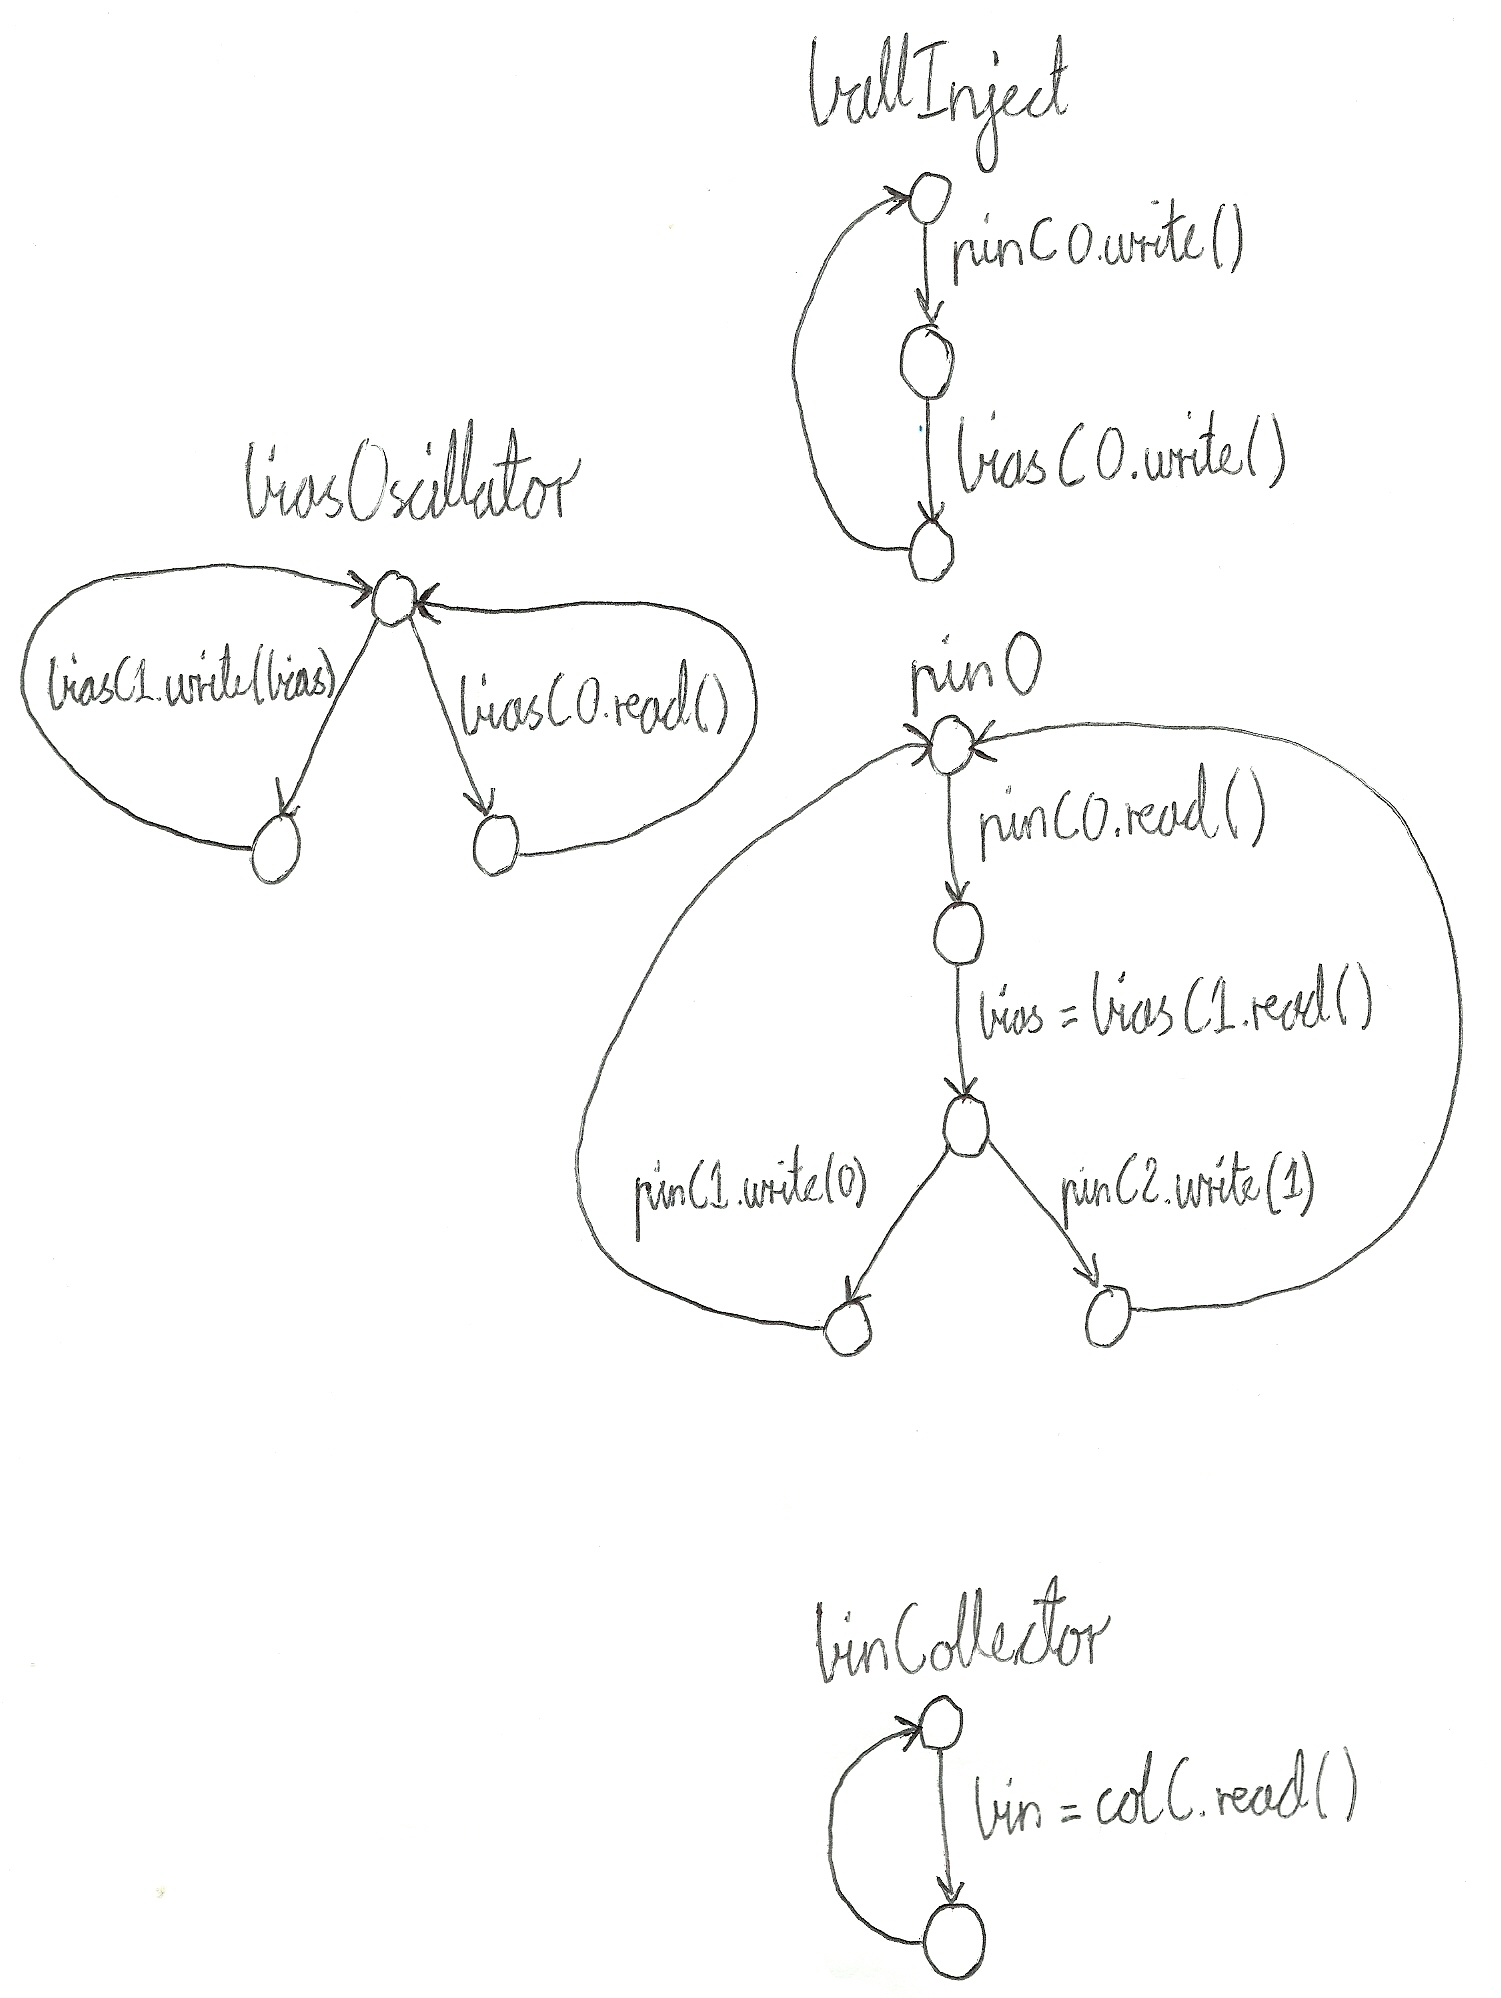
\includegraphics[width=\textwidth]{program_network.jpg}
    \caption{Program network}
    \label{fig:program_network}
\end{figure}

\section{Initiation}
All processes of the network are initialized and run in parallel by the use of
the \texttt{beanMachine} function, which is able to start a network of $n$
layers. The network can either be terminated by the \texttt{count} or the
\texttt{inject} method at a stopping condition count $s$. The
\texttt{ballInject} process is the process which initiates the entire network by
starting to inject balls.

\section{Termination}
When using the \texttt{inject} termination, the \texttt{ballInject} process loops
for $s$ iterations (injects $s$ balls) and then retires from the channel
$pinC0$. The retire exception will propagate down through the pins. Since all
pin channels are many2one, all writers have to retire before the propagation
continues and hence ensuring that all balls are propagated before closing the
network. At the bottom layer the \texttt{binCollector} likewise has a many2one
input channel, which requires all pins to retire before the collector retires
itself. Once this happens, the bin collector poisons a reading end of the biasC0
channel and hence the entire network is shut down.

When using the \texttt{count} termination, the \texttt{ballInject} process loops
infinitely and the termination is handled by the \texttt{binCollector} process.
Once a total of $s$ balls/beans have been counted by the \texttt{binCollector},
the counting stops and the \texttt{colC} and \texttt{biasC0} channels are poisioned
and hence all the pins as well as the injector will die once the poison
propagates upwards.

Both these termination schemes ensure that we have exactly $s$ balls counted at
the \texttt{binCollector} once it shuts down, which the experiments of running a
network of $n = 50$ layers, $s = 1000$ and using each of the stopping conditions
verify by having totals of exactly 1000 balls at termination.

\clearpage
\includepdf[pages=-]{codelisting.pdf}

\end{document}

